%    Latex Template for ACA 2015
%%%%%%%%%%%%%%%%%%%%%%%%%%%%%%%%%%%%%%%%
%    DO NOT CHANGE THE SETTINGS BELOW
%%%%%%%%%%%%%%%%%%%%%%%%%%%%%%%%%%%%%%%%
\documentclass[11pt]{article}
\usepackage{epsfig}
\usepackage{graphicx}
\usepackage[latin1]{inputenc}
\usepackage[T1]{fontenc}
\usepackage{mathptmx}
\usepackage{url}



%%%%%%%%%%%%%%%%%%%%%%%%%%%%%%%%%%%%%%%%%%%%%%%%%%%%%%%%%%%%%
%%%%%%%%%%% Begin of Autors preabmule settings %%%%%%%%%%%%%%

\usepackage{amsmath, amsfonts, amsthm}
\usepackage{epigraph}
\usepackage{float}

\theoremstyle{definition}
\newtheorem{defin}{Definition}


\newcommand{\ds}{\displaystyle}
\newcommand{\R}{\mathbb{R}}
\newcommand{\dx}{\,\mathrm{d}}

%%%%%%%%%%% End of Autors preabmule settings %%%%%%%%%%%%%%
%%%%%%%%%%%%%%%%%%%%%%%%%%%%%%%%%%%%%%%%%%%%%%%%%%%%%%%%%%%




\begin{document}



%%%%%%%%%%%%%%%%%%%%%%%%
%%%%%%%%%%%%%%%%%%%%%%%%%%%%%%%%%%%%%%%%
%    DO NOT CHANGE THE SETTINGS ABOVE
%%%%%%%%%%%%%%%%%%%%%%%%%%%%%%%%%%%%%%%%
%





\vspace{-0.8cm}
\begin{flushleft}
\Large \textbf{\noindent
%%% PLEASE INSERT THE TITLE OF YOUR TALK HERE %%%%%%%
Visualization of simplex method with Mathematica}
%%%%%%%%%%%%%%%%%%%%%%%%%%%%%%%%%%%%%%%%%%%%%%%%%%%%%%%%
\\
%%%%%%%%%%%%%%%%%%%%%%%%%%%%%%
\vspace{0.5cm}
\normalsize
 %%%%%%             NAMES OF AUTHORS         %%%%%%
 %%%%%% NAME OF SPEAKER SHOULD BE UNDERLINED %%%%%%%%%
\normalsize{
 %%%%%% FOR EXAMPLE %%%%%
\underline{ W{\l}odzimierz Wojas$^1$}, \underline{Jan Krupa}$^2$
 %%%%%%%%%%%%%%%%%%%%%%%%
} \\
\vspace{5mm}
\textit{\footnotesize
 %%%%%% AFFILIATION OF AUTHORS %%%%%%
$^1$ Warsaw University of Life Sciences (SGGW), Poland, {\tt wlodzimierz\_wojas@sggw.pl}\\
$^2$ Warsaw University of Life Sciences (SGGW), Poland, {\tt jan\_krupa@sggw.pl}\\
 %%%%%%%%%%%%%%%%%%%%%%%%%%%%%%%%%%%%%
}
\end{flushleft}

Simplex algorithm is taught at universities in framework of different academic courses, for example Linear Programming, Mathematical Programming or Operation Research. One aspect of the teaching of this algorithm is to present a geometric interpretation of simplex steps. Some attempts to visualization simplex method using CAS were taken in papers  \cite{Stan, Liu, Bulmer}. In this article, the authors propose some new approach to this subject through the use of expanded Simplex Tableau. This Tableau, for each of simplex step contains: current simplex table for this step, graph of feasible region for standard form of LP problem with current vertex of simplex path, current level set of objective function corresponding to this step (hyperplanes : lines in 2D, planes in 3D), axis with current value of objective function for this step. The presentation was prepared using Mathematica. We present examples for 2D and 3D feasible regions. One of them is presented below.

\quad

\noindent
{\bf Example.}

\noindent
Let us visualize simplex steps for the following LP problem in standard form (in $\mathbb{R}^2$):
  \begin{alignat*}{4}
    \text{Maximize\quad}   &\rlap{$z=3x_1+2x_2$} &&&&&&  \\
    \text{Subject to\quad} &&x_1&{}-{}&3x_2&\leq{}&2&\\
                        &&x_1&{}-{}&x_2&\leq{}&4&\\
                        &&5x_1&{}-{}&x_2&\leq& 36&\\
                        &&-4x_1&{}+{}&\frac{5}{2}x_2&\leq{}& 5&\\
                        &&-x_1&{}+{}&4x_2&\leq& 16&\\
                        && & &x_2&\leq{}&  9&\\
                        & \rlap{$x_i \geq 0 \mbox{  for   }
                         i = 1, 2$.} &&&&&&
  \end{alignat*}


Corresponding to it canonical form is:
\begin{alignat*}{10}
    \text{Maximize}\quad   &\rlap{$z=3x_1+2x_2$} \\
    \text{Subject to}\quad &&x_1&-{}&3x_2&+{}&x_3& &&&&&&&&&& ={}& 2\\
                           &&x_1&-{}&x_2& & &+{}&x_4& &&&&&&&&={}& 4\\
                           &&5x_1&-{}&x_2&&&&&+{}&x_5& &&&&&&= &36\\
                           &&-4x_1&+{}&\frac{5}{2}x_2&&&&&&&+{}&x_6&&&&&={}& 5\\
                           &&-x_1&+{}&4x_2&&&&&&&&&+{}&x_7& &&={}& 16\\
                           &&&&x_2&&&&&&&&&&&+{}&x_8& ={}&  9\\
                           &\rlap{$x_i\geq 0 \mbox{  for   } i=1,2,\ldots,8$}
 \end{alignat*}


\noindent
Feasible region for this LP problem (in standard form) is presented in each Figure 1--5. It is convex polyhedral set with vertices at: $v_1=(0,0),  v_2=(2,0), v_3=(5,1),v_4=(8,4),v_5=(9,9),v_6=(6.5,9),v_7=(2.5,6),v_8=(0,2)$.
In each  Figure 1--5 we present expanded Simplex Tableau for subsequent vertices of simplex path.



\begin{figure}[H]
\begin{center}
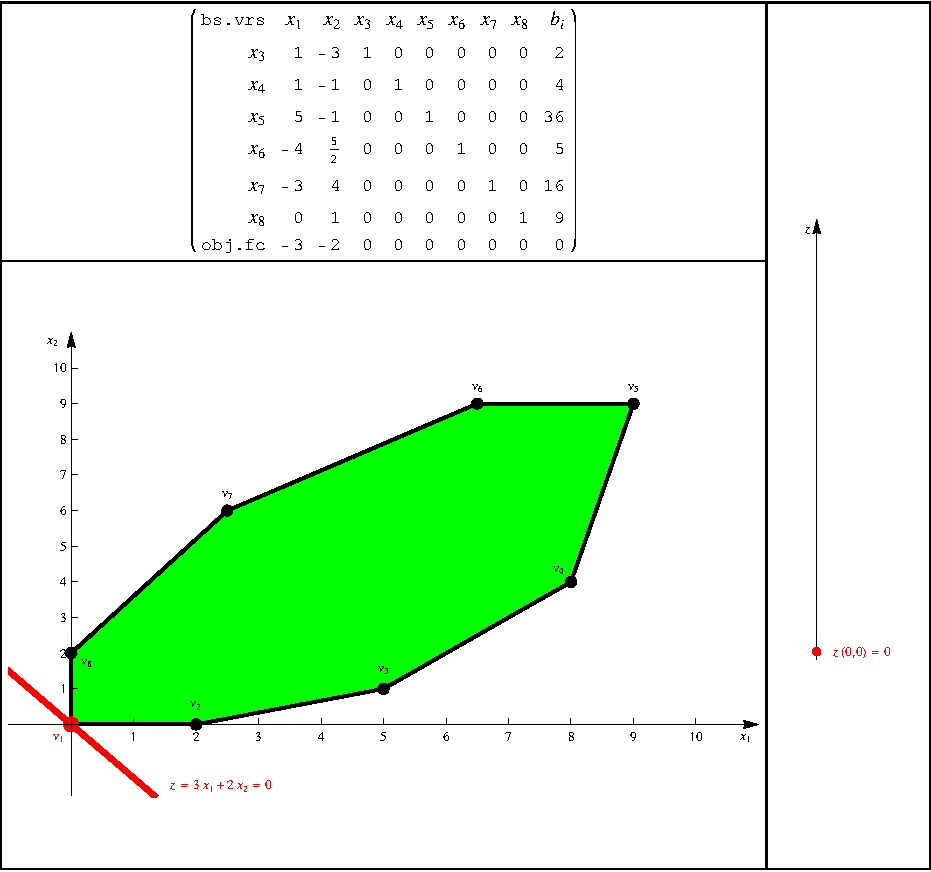
\includegraphics[scale=0.8]{tab0.pdf}
\caption{First expanded Simplex Tableau.}
\label{fig:0}
\end{center}
\end{figure}

\begin{figure}[H]
\begin{center}
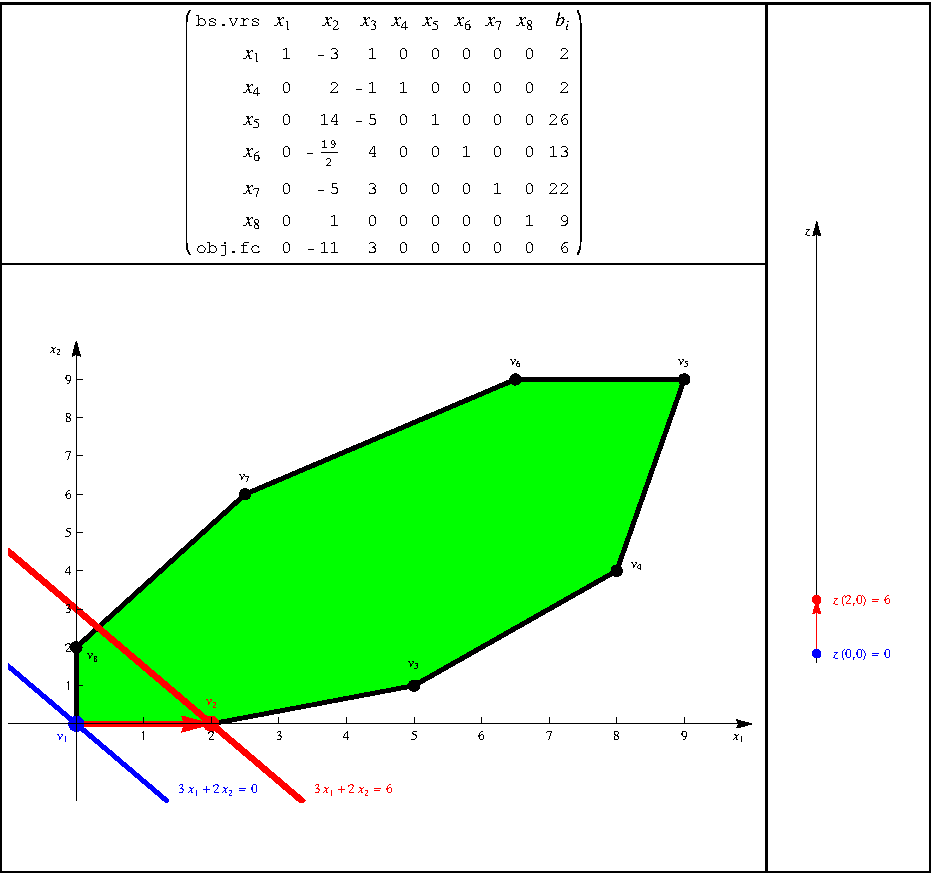
\includegraphics[scale=0.8]{tab1.pdf}
\caption{Second expanded Simplex Tableau.}
\label{fig:1}
\end{center}
\end{figure}


\begin{figure}[H]
\begin{center}
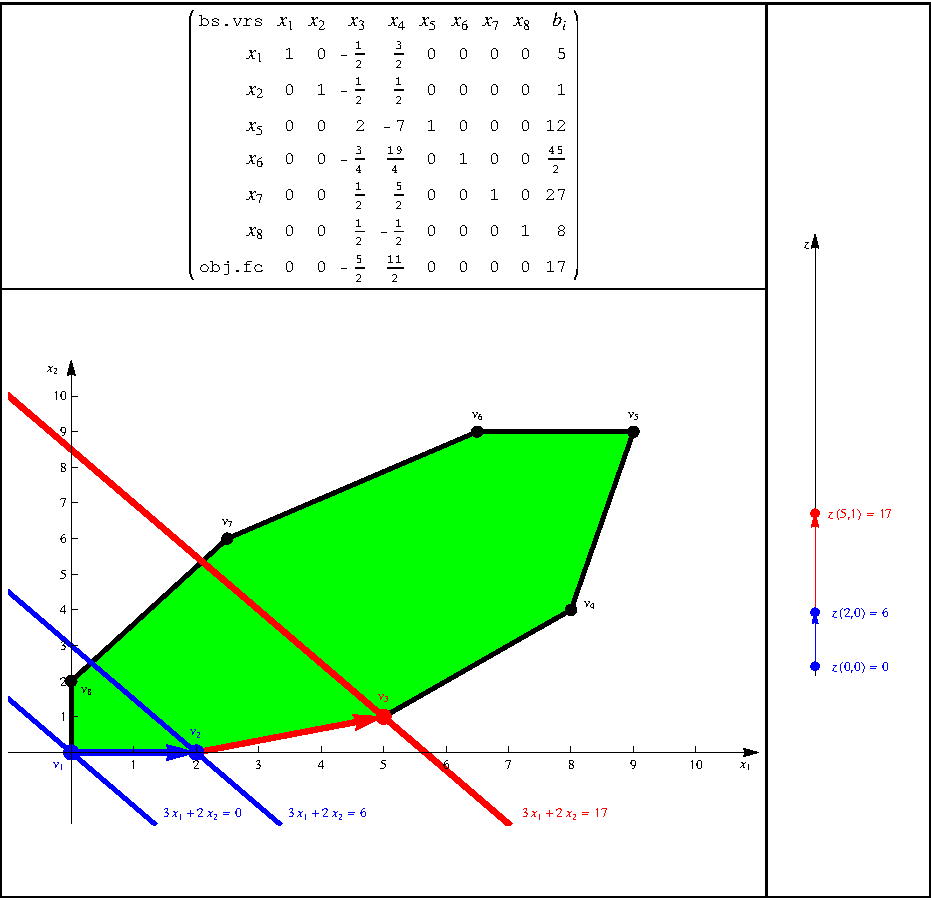
\includegraphics[scale=0.8]{tab2.pdf}
\caption{Third expanded Simplex Tableau.}
\label{fig:2}
\end{center}
\end{figure}

\begin{figure}[H]
\begin{center}
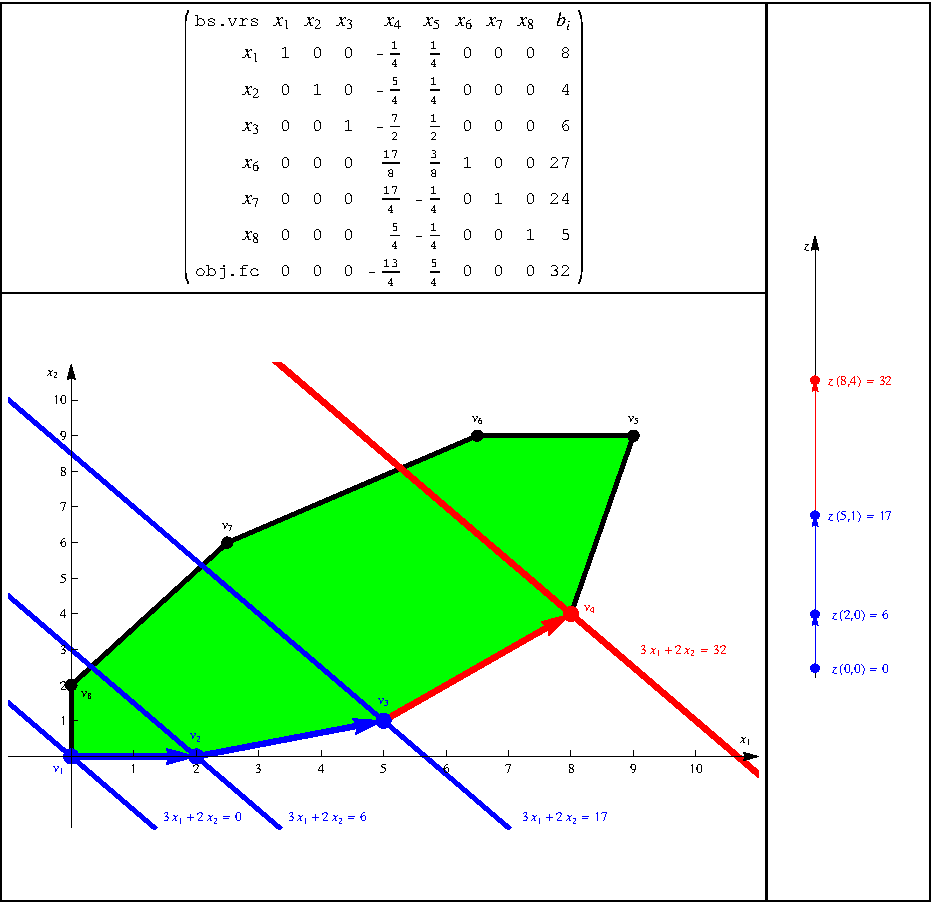
\includegraphics[scale=0.8]{tab3.pdf}
\caption{Forth expanded Simplex Tableau.}
\label{fig:3}
\end{center}
\end{figure}

\begin{figure}[H]
\begin{center}
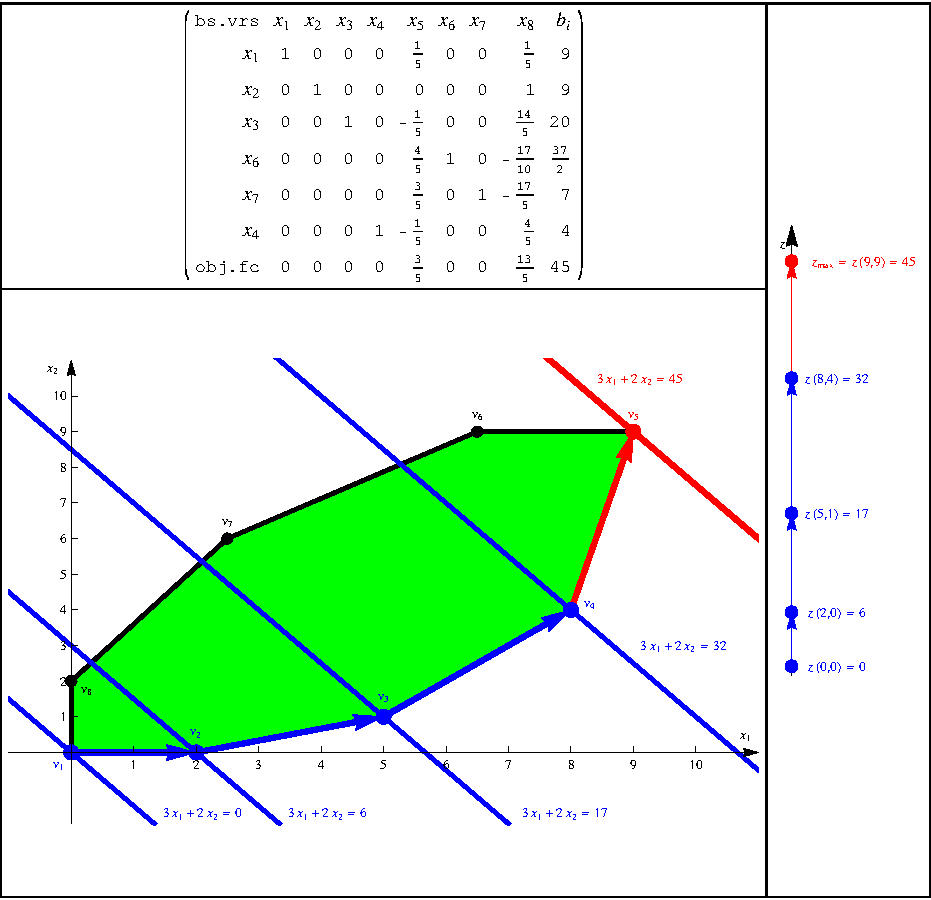
\includegraphics[scale=0.8]{tab4.pdf}
\caption{Fifth expanded Simplex Tableau.}
\label{fig:4}
\end{center}
\end{figure}


The fifth expanded Simplex Tableau is optimal. We have: $z_{\mathrm{max}}=z(9,9)=45$.



%%%%%%%%%%%%%%%%%%%%%%%%%%%%%%%%%%%%%%%%
%% BIBLIOGRAPHY
%%%%%%%%%%%%%%%%%%%%%%%%%%%%%%%%%%%%%%%%
\begin{thebibliography}{00}
\addcontentsline{toc}{chapter}{References}
\setlength{\itemsep}{-1mm}
\footnotesize
\bibitem{Stan} Predrag S. Stanimirovic, Marko D. Petkovic, Milan Lj. Zlatanovic, \textit{Visualization in optimization with Mathematica}, Filomat, 2009 23(2):68-81
\bibitem{Kol} Bernard Kolman and Robert E. Beck, \textit{Elementary Linear Programming with Applications}, 2\textsuperscript{nd} ed., Academic Press, (1995)
\bibitem{Luen}  David G. Luenberger, \textit{Linear and Nonlinear Programming}, 3\textsuperscript{rd} ed., Springer,  (2010)
\bibitem{Liu} D. K. Liu, S.D. Huang, T.A. Brown, \textit{Supporting Teaching and Learning of Optimisation Algorithms with Visualisation Techniques}, Proceedings of the 2007 AaeE Conference, Melbourne, (2007)
\bibitem{Bulmer} Michael Bulmer  and Michael Carter, \textit{Integer programming with Mathematica}, The Mathematica Journal 1996, Miller Freeman Publication
\bibitem{Ruskeepa} H. Ruskeepa \textit{Mathematica Navigator: Graphics and Methods of applied Mathematics.}
Academic Press, Boston (2005)
\bibitem{Wolfram}
S. Wolfram  \textit{The Mathematica Book.} Wolfram Media/ Cambridge University Press (1996)
\end{thebibliography}
\normalsize

\end{document}
